\documentclass{article}

\usepackage{iclr2026_conference,times}

\input{math_commands.tex}

\usepackage{amsmath}
\usepackage{amssymb}
\usepackage{array}
\usepackage{booktabs}
\usepackage{multirow}
\usepackage{pifont}
\usepackage{xcolor}
\usepackage{hyperref}
\usepackage{url}
\usepackage{tikz}
\usetikzlibrary{arrows.meta,positioning,fit,backgrounds,calc}

% ---- project macros ----
\newcommand{\method}{HSE}
\newcommand{\skillrepo}{SkillRepo}
\newcommand{\tbd}{\textcolor{gray}{--}}            % unfilled numeric cell
\newcommand{\dpos}[1]{\textcolor{teal!70!black}{$+#1$}}
\newcommand{\dneg}[1]{\textcolor{red!70!black}{$-#1$}}
\newcolumntype{L}[1]{>{\raggedright\arraybackslash}p{#1}}
\newcolumntype{C}[1]{>{\centering\arraybackslash}p{#1}}

% ---- shared tikz styles for the pipeline / boundary figures ----
\tikzset{
  stage/.style={draw, rounded corners=2pt, align=center, font=\small,
                minimum height=9mm, inner sep=4pt, fill=blue!4},
  gate/.style={draw, rounded corners=2pt, align=center, font=\footnotesize,
               fill=orange!12, inner sep=3pt},
  flow/.style={-{Stealth[length=2.2mm]}, thick},
}

\title{Hierarchical Skill Evolution for Software-Engineering Agents}

% Anonymous submission. Uncomment \iclrfinalcopy only for camera-ready.
\author{Anonymous authors}

% \iclrfinalcopy
\begin{document}

\maketitle

\begin{abstract}
Software-engineering agents generate rich traces, including issue
interpretations, file searches, edits, test runs, failures, and recoveries,
that are discarded after each benchmark trial. Recycling these traces into
reusable text skills is an attractive way to let a frozen agent accumulate
experience, but it is also where most systems introduce leakage: raw trace
retrieval carries task-specific solutions into future prompts, and one-shot
``summarize the trajectory'' pipelines emit over-specific or actively harmful
instructions that no one audits. Either way, apparent gains come from
memorization or noise rather than transfer. We present \method{}, a
verifier-grounded framework that evolves external skills for \emph{frozen}
coding agents while making leakage structurally hard. \method{} refuses to call
every trace artifact a skill: it separates single-task evidence from reusable
skills, promotes evidence through a hierarchy of repo-level and cross-repo
behavior skills, and trains separate Skill Writer and Skill Evaluator
policies behind a fixed harness policy. The design is built around one hard
information boundary. During SWEGym training the official verifier supplies
outcome labels, evaluator calibration, and validation gates; at downstream
evaluation the verifier never touches the update path, so no hidden test, gold
patch, or future outcome may alter a skill. We instantiate the framework in a
runnable system (Pi harness, OpenAI-compatible models served from our own
self-hosted deployment, versioned skill archives with promotion logs and
validation gates) and specify an evaluation protocol over GLM-5.2 under two
agent harnesses, Pi and Claude-style, that isolates harness transfer, with
SWE-bench Verified and DeepSWE as in-domain targets, all under a shared
sandbox and acceptance rule.
\end{abstract}

\section{Introduction}

Large language model agents can repair real software bugs: they read a
repository, edit code, run tests, and recover from failures. Every one of those
attempts---successful or not---produces information about how to localize, edit,
validate, and recover on the next task. Almost all of it is thrown away the
moment the benchmark scores the trial. Recycling it into external
\emph{skills}---compact textual procedures injected into future prompts---is an
attractive way to make a frozen agent better without retraining its weights.

The attraction hides a trap. A raw trajectory is full of things that must not
leak forward: concrete file paths, the exact shape of a gold patch, transient
environment errors, and incidental identifiers of the benchmark instance. Inject
those into a future prompt and the system improves by \emph{memorization}, not
transfer---and on a held-out benchmark this is indistinguishable from progress
until someone audits the prompt. The opposite failure is just as common: a
one-shot ``summarize the trajectory into advice'' step yields instructions like
``run focused tests'' that are too generic to change behavior, or over-specific
rules that fire on the wrong task and cause regressions. We argue that most
trace-to-skill pipelines sit on one of these two failure modes and report the
resulting numbers as if they measured transfer.

The question we take seriously is therefore: \emph{can a coding-agent system
learn reusable software-engineering skills from training-time verifier feedback
without using test-time verifier feedback and without leaking task-specific
solutions?} Answering it requires more than a better summarizer. It requires (i)
a disciplined notion of what is allowed to become a transferable skill, and (ii)
a hard, auditable boundary on when the verifier may influence memory.

We propose \method{}, \textbf{hierarchical skill evolution}. The central design
commitment is restraint: \emph{not every trace artifact is a skill}. A task
attempt first becomes \emph{task evidence}---a structured record of public
signals (touched and edited paths, test commands, diagnostics, selected skills,
failure signatures, verifier outcome). Task evidence is never rendered as a
deployed skill. A Skill Writer drafts a repo-level skill only from \emph{multiple}
evidence records in the \emph{same} repository, and a failure-mode skill only
from patterns that \emph{recur across} repositories---localization drift, weak
validation, no-diff exits, timeout recovery. A Skill Evaluator then scores each
candidate for utility, support, and risk and decides whether to accept, reject,
revise, or retain it as memory-only evidence. Every upward step is gated; a
single lucky trace cannot mint a global skill.

The boundary is the second commitment, and it is hard rather than aspirational.
SWEGym verifiers are available at training time, so we use them to label
outcomes, calibrate the evaluator, and gate candidate states on a repo-isolated
validation split. On SWE-bench Verified and other downstream benchmarks, no
official verifier label, hidden test result, gold patch, or future task outcome
may influence a skill update---full stop. This is what makes a transfer claim on
those benchmarks meaningful rather than a restatement of leaked supervision.

\paragraph{Contributions.}
\begin{itemize}
    \item We recast software-agent skill evolution as a hierarchical,
    evidence-gated process that cleanly separates task evidence, repo-level
    skills, cross-repo failure-mode skills, and the writer/evaluator policies
    that produce and police them.
    \item We define a verifier-boundary protocol that licenses training-time use
    of SWEGym verifier outcomes while forbidding any verifier signal on the
    test-time update path, turning leakage from a reviewer's worry into a
    structural property of the system.
    \item We instantiate the framework end to end for the Pi coding-agent
    harness with an OpenAI-compatible model interface, Harbor/E2B execution,
    versioned skill archives, promotion logs, validation gates, and a
    deterministic evaluator shell that can be swapped for a learned policy
    without changing the loop contract.
    \item We specify an evaluation protocol over a GLM-5.2/GPT-5.5
    $\times$ Pi/Claude-style matrix that separates within-cell evolution, model
    transfer, and harness transfer across SWE-bench Verified, DeepSWE, and an
    out-of-domain Terminal-Bench 2.0/2.1 extrapolation, treating exact-task
    memory only as an explicitly labeled adaptation upper bound.
\end{itemize}

\section{Problem Setting}

\paragraph{Tasks and agents.}
A software-engineering task $x$ consists of a natural-language issue, a
repository snapshot, and a public execution environment. A frozen coding agent
$M$ interacts with a harness $H$ by issuing file reads, searches, edits, shell
commands, and a final answer. A trajectory $\tau$ records the observable history:
prompts, tool calls, outputs, diffs, public tests, and runtime diagnostics. $M$
and $H$ are fixed throughout; the only thing that evolves is the external skill
state.

\paragraph{Training-time verifier.}
During SWEGym training we hold a verifier $V$ mapping a completed trial to a
reward $r \in \{0,1\}$ or a diagnostic outcome. $V$ supervises training-time
labels and validation gates. It is deliberately \emph{not} a writer of skills
and \emph{not} a source of hidden solutions. At downstream test time $V$ is
unavailable for any memory update; it is invoked only after the protocol
completes, to report final benchmark scores.

\paragraph{Skill state.}
The external state $S$ holds structured evidence and accepted skills in four
deployed categories:
\begin{itemize}
    \item \textbf{Task evidence} records what happened on one task. It is not a
    reusable skill and is never deployed as one.
    \item \textbf{Repo skills} summarize repeated, evidence-gated procedures
    within a single repository.
    \item \textbf{Failure-mode skills} summarize cross-repo recovery strategies
    for recurring agent failures. These are the primary transferable artifact.
    \item \textbf{General seed skills} provide weak process priors for common
    stages (reproduce, localize, edit, validate, recover).
\end{itemize}
The writer policy $\pi_w$ drafts evidence summaries and candidate skills; the
evaluator policy $\pi_e$ assigns decisions, proxy rewards, confidence, and risk
flags.

\section{Hierarchical Skill Evolution}

\subsection{A hierarchy with different update clocks}

\method{} updates different abstraction levels at different rates. Low levels
change quickly because a mistake there touches only local evidence; high levels
change slowly because a mistake there propagates into every future task.
Table~\ref{tab:levels} lists the objects, their clocks, and the evidence each
promotion requires.

\begin{table}[t]
\caption{Skill-evolution objects and update clocks. The main experiments freeze
all training-derived transferable state before any downstream evaluation.}
\label{tab:levels}
\begin{center}
\small
\begin{tabular}{@{}c L{0.24\linewidth} L{0.24\linewidth} L{0.30\linewidth}@{}}
\toprule
Level & Object & Update clock & Evidence requirement \\
\midrule
L0 & Rollout trace & Every task attempt & Public trajectory and runtime outputs \\
L1 & Task evidence & Every task attempt & One task trace; verifier label (train only) \\
L2 & Repo skill candidate & Same-repo batch & Multiple evidence records, one repo \\
L3 & Behavior candidate & Cross-repo trigger & Repeated repo summaries across repos \\
L4 & Skill Writer policy & Slow policy window & Aggregated accept/reject histories \\
L5 & Skill Evaluator policy & Slow policy window & Verifier-calibrated false accepts/rejects \\
\bottomrule
\end{tabular}
\end{center}
\end{table}

Task evidence stores public fields only: task id, repo, problem summary,
reward, previous reward, case label, exception type, selected skills, touched and
edited paths, public test commands, failure signature, and diagnostic signals.
It feeds higher-level aggregation but is never exported as a reusable
\texttt{SKILL.md}.

\begin{figure}[t]
\centering
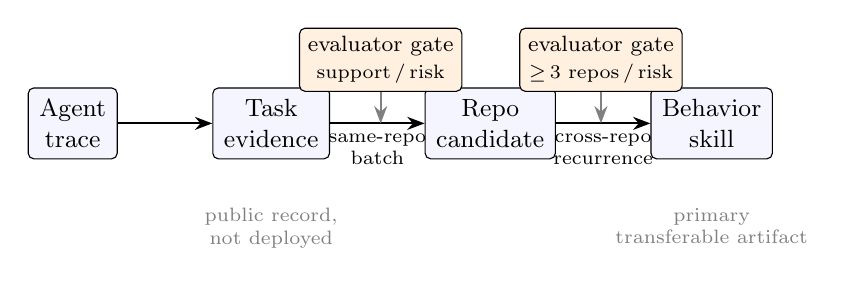
\begin{tikzpicture}[node distance=7mm and 12mm]
  \node[stage] (trace) {Agent\\trace};
  \node[stage, right=of trace] (evid) {Task\\evidence};
  \node[stage, right=of evid] (repo) {Repo\\candidate};
  \node[stage, right=of repo] (fail) {Behavior\\skill};
  % gates on the arrows
  \node[gate, above=4mm of $(evid)!0.5!(repo)$] (g1) {evaluator gate\\\scriptsize support\,/\,risk};
  \node[gate, above=4mm of $(repo)!0.5!(fail)$] (g2) {evaluator gate\\\scriptsize $\geq$\,3 repos\,/\,risk};
  \draw[flow] (trace) -- (evid);
  \draw[flow] (evid) -- node[below, font=\scriptsize, align=center]{same-repo\\batch} (repo);
  \draw[flow] (repo) -- node[below, font=\scriptsize, align=center]{cross-repo\\recurrence} (fail);
  \draw[flow, gray] (g1) -- ($(evid)!0.5!(repo)$);
  \draw[flow, gray] (g2) -- ($(repo)!0.5!(fail)$);
  \node[below=5mm of evid, font=\scriptsize, text width=2.4cm, align=center, gray]
    {public record,\\not deployed};
  \node[below=5mm of fail, font=\scriptsize, text width=2.6cm, align=center, gray]
    {primary\\transferable artifact};
\end{tikzpicture}
\caption{The promotion pipeline. A trace becomes task evidence, then a repo-level
candidate, then a cross-repo behavior skill. Task evidence is never deployed
directly; each upward step passes an evaluator gate that checks support, risk,
and validation. Repo promotion needs repeated same-repo evidence; behavior
promotion needs at least three distinct repositories.}
\label{fig:pipeline}
\end{figure}

\subsection{Writer and evaluator: generation versus gatekeeping}

The writer turns clusters of evidence into structured candidates. From a cluster
of same-repo evidence it emits a repo candidate with fields name, trigger,
evidence gate, actions, validation hint, abort condition, and support summary.
From a cross-repo cluster it emits a process-level behavior candidate with a
failure signature, trigger, actions, stop condition, and support summary:
\[
c_{\mathrm{repo}} = f_w(E_{\mathrm{repo}}), \qquad
c_{\mathrm{fail}} = f_w(E_{\mathrm{cross\text{-}repo}}).
\]
The structure is not decoration: it forces every candidate to expose its trigger,
support, actions, and risks so the evaluator can inspect them before anything is
deployed.

The evaluator is the gatekeeper that separates generation from deployment:
\[
\pi_e(c, E) \rightarrow (d, \hat r, \rho, z),
\]
with decision $d \in \{\textsc{accept}, \textsc{reject}, \textsc{revise},
\textsc{memory-only}\}$, proxy reward $\hat r$, confidence $\rho$, and risk flags
$z$. Hard safety risks (hidden verifier details, oracle or exact patches,
task-id memorization, private sandbox paths) force rejection regardless of
apparent utility. Repo candidates require repeated same-repo support; behavior
candidates require support from multiple distinct repositories. A single repo can
never originate a behavior skill.

We deliberately ship a \emph{deterministic} evaluator shell with explicit
thresholds and risk checks. This is an interface choice, not a limitation: it
makes the accept/reject contract auditable today, while exposing exactly the same
call signature that a learned evaluator, trained on SWEGym calibration
events, can later occupy without disturbing the rest of the loop.

\subsection{A fixed harness policy the learned policies cannot rewrite}

The learned writer and evaluator are explicitly forbidden from inventing their
own reward labels, update clocks, or promotion budgets. A fixed harness policy
maps verifier transitions and runtime diagnostics to case labels. A
\textbf{strong positive} is a previous attempt that failed and a current
attempt that passed; a \textbf{weak positive} is a current attempt that passed
without a paired improvement, or a previously passing attempt that stays
passing. A \textbf{strong negative} is a previous attempt that passed and a
current attempt that failed; a \textbf{weak negative} is a current attempt that
failed without a paired regression. A \textbf{diagnostic} covers missing reward,
timeout, setup error, verifier error, sandbox failure, or provider/runtime
failure. Cold-start solved traces are weak positives; unsolved traces are weak
negatives unless a diagnostic is present. Strong positives may add support to a
candidate but cannot by themselves create a global skill. Strong negatives
prioritize rollback, trigger narrowing, and evaluator false-accept penalties.
Diagnostics are kept out of semantic edit skills entirely and used only to
shape runtime or recover/validate safeguards.

\subsection{Training loop and the verifier boundary}

Training alternates rollout, evidence extraction, candidate generation, evaluator
gating, and validation (Figure~\ref{fig:verifier-boundary}, top lane). The
verifier supervises case labels, calibrates the evaluator, and gates candidate
states, and nothing more. At downstream evaluation (bottom lane) the writer,
evaluator, and transferable skills are frozen and only public trace signals enter
the update path.

\begin{figure}[t]
\centering
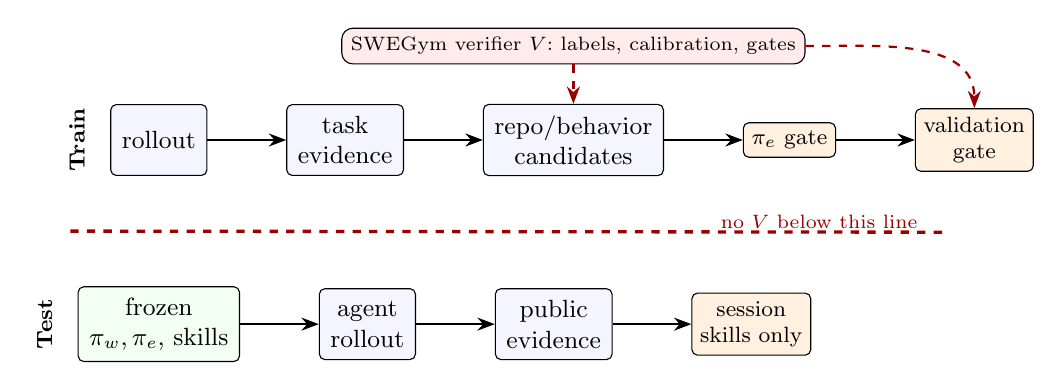
\begin{tikzpicture}[node distance=6mm and 10mm]
  % training lane
  \node[stage, fill=blue!4] (r1) {rollout};
  \node[stage, right=of r1] (e1) {task\\evidence};
  \node[stage, right=of e1] (c1) {repo/behavior\\candidates};
  \node[gate, right=of c1] (g1) {$\pi_e$ gate};
  \node[gate, right=of g1] (v1) {validation\\gate};
  \draw[flow] (r1)--(e1); \draw[flow] (e1)--(c1); \draw[flow] (c1)--(g1); \draw[flow] (g1)--(v1);
  \node[draw, fill=red!8, rounded corners, font=\scriptsize, above=5mm of c1] (ver)
    {SWEGym verifier $V$:\ labels, calibration, gates};
  \draw[flow, red!60!black, dashed] (ver) -- (c1);
  \draw[flow, red!60!black, dashed] (ver.east) to[out=0,in=90] (v1.north);
  \node[left=2mm of r1, font=\footnotesize\bfseries, rotate=90, anchor=south] {Train};

  % downstream lane
  \node[stage, fill=green!5, below=14mm of r1] (r2) {frozen\\$\pi_w,\pi_e$, skills};
  \node[stage, right=of r2] (a2) {agent\\rollout};
  \node[stage, right=of a2] (p2) {public\\evidence};
  \node[gate, right=of p2] (s2) {session\\skills only};
  \draw[flow] (r2)--(a2); \draw[flow] (a2)--(p2); \draw[flow] (p2)--(s2);
  \node[left=2mm of r2, font=\footnotesize\bfseries, rotate=90, anchor=south] {Test};
  % the boundary
  \draw[red!60!black, very thick, dashed] ($(r1.south west)!0.5!(r2.north west)+(-0.3,0)$)
     -- ($(v1.south east)!0.5!(s2.north east)+(0.3,0)$);
  \node[red!60!black, font=\scriptsize] at ($(s2.north east)+(0.1,0.9)$) {no $V$ below this line};
\end{tikzpicture}
\caption{The verifier boundary. \textbf{Top (train):} verifier $V$ supplies
outcome labels, evaluator calibration, and validation gates. \textbf{Bottom
(test):} the writer, evaluator, and transferable skills are frozen and only
public trace signals update memory. $V$ appears in the training lane and in final
reporting only---never on the downstream update path.}
\label{fig:verifier-boundary}
\end{figure}

\paragraph{Default update hyperparameters.}
Unless stated otherwise, repo updates use same-repo batches of 5 evidence events,
behavior updates trigger every 4 repo updates, a behavior promotion
requires at least 3 supporting repositories, and policy updates are capped at 3
bullet edits per policy window. Each repo batch emits at most one repo candidate;
each behavior trigger promotes at most two accepted behavior skills.
These values are the harness defaults and are treated as fixed protocol
hyperparameters, not tuned per benchmark.

\subsection{Validation gate}

Candidate skill states are scored on a repo-isolated SWEGym validation set via
\[
\mathrm{effective\_resolved\_rate}
= \frac{\#\,\text{resolved valid trials}}{\#\,\text{effective valid trials}},
\qquad
\mathrm{diagnostic\_rate}
= \frac{\#\,\text{diagnostic trials}}{\#\,\text{total trials}}.
\]
A candidate state is accepted only if it has enough effective validation trials,
stays under the diagnostic-rate threshold, and does not regress beyond a fixed
tolerance relative to the current accepted state. Otherwise the candidate version
is rejected or rolled back and the decision is logged. The gate exists precisely
to stop a plausible-looking candidate from silently trading pass rate for
regressions.

\section{Experiments}

We report the experimental \emph{settings} in full and leave numeric cells as
\tbd{} until the corresponding runs complete; every table is structured so a
reader sees the baseline, the \method{} result, and their difference side by
side rather than as disconnected rows.

\subsection{Benchmarks}

\paragraph{In-domain targets.}
The primary downstream benchmark is \textbf{SWE-bench Verified}, the
human-verified subset of SWE-bench. We additionally evaluate on \textbf{DeepSWE},
a harder issue-resolution suite, to test that gains are not an artifact of a
single benchmark. On both, no official verifier label, hidden test, or gold patch
enters the skill-update path during the evaluated run; the official verifier is
invoked only afterward to report resolved count and rate.

\paragraph{Out-of-domain extrapolation.}
We treat \textbf{Terminal-Bench 2.0 and 2.1} as an extrapolation test: the agent
faces general command-line tasks rather than repository patching, but runs
through the same Harbor/E2B wrapper. This isolates whether the cross-repo
failure-mode skills---reproduce, localize, validate, recover---survive a shift
away from the issue-resolution distribution they were evolved on, or whether they
silently degrade.

\paragraph{Evolution source.}
All transferable state is evolved on a 500-task SWEGym subset under a
repo-isolated split: validation repositories are held out from training, with the
validation size chosen closest to 5\% of the subset, yielding 474 training and 26
validation tasks. The SWEGym verifier is available only in this phase.

\subsection{Models and harnesses}

\paragraph{Executor matrix.}
We evaluate two executor models, GLM-5.2 (\texttt{glm52}) and GPT-5.5, each under
two agent harnesses, Pi and a Claude-style coding-agent harness. All four cells
share the same Harbor/E2B sandbox interface, task selection, task ordering,
timeout budget, validation gate, and no-test-verifier update rule. Where model
APIs differ we route through one OpenAI-compatible provider abstraction and record
the endpoint type in the run config.

\paragraph{Three transfer questions.}
The $2{\times}2$ matrix isolates three questions that prior work routinely
conflates. \textbf{Model transfer}: skills and policies evolved with one model are
evaluated with the other under a fixed harness. \textbf{Harness transfer}: skills
evolved under one harness are evaluated under the other with a fixed model.
\textbf{Joint transfer}: both model and harness change between evolution and
evaluation. We report each separately from within-cell evolution, where evolution
and evaluation share the same cell.

\paragraph{Controls.}
The tool surface is fixed within each harness family (read, write, edit, bash,
grep, find, ls). Prompts may differ between Pi and Claude-style harnesses, but
task order, sandbox resources, retry policy, and acceptance rules are held fixed.
Every run logs the active skill version, the source and target cell, selected
skills, runtime diagnostics, verifier reports, and score reports, so any reported
delta is attributable to the skill state rather than to a moving control.

\subsection{Protocols}

\begin{table}[t]
\caption{Evaluation protocols. Exact-task skills are reported only as an
adaptation upper bound and never used to support a transfer claim.}
\label{tab:protocols}
\begin{center}
\small
\begin{tabular}{@{}L{0.30\linewidth} C{0.12\linewidth} C{0.14\linewidth} L{0.32\linewidth}@{}}
\toprule
Setting & Exact task memory & Test-time update & Purpose \\
\midrule
No Skills & \ding{55} & \ding{55} & Frozen-agent baseline \\
Public SWE Skills & \ding{55} & \ding{55} & Static public-skill baseline \\
Raw Trace Retrieval & \ding{55} & \ding{55} & Does raw trajectory memory suffice? \\
One-shot StageSkill & \ding{55} & \ding{55} & Ungated trace-to-skill summarization \\
Frozen Failure Skills & \ding{55} & \ding{55} & SWEGym-trained transferable skills \\
Frozen $\pi_w/\pi_e$ + online repo & \ding{55} & public only & Verifier-free online evolution \\
Same-budget Retry & \ding{55} & \ding{55} & Controls for extra attempts/compute \\
Exact Task Skills & \checkmark & optional & Adaptation upper bound only \\
\bottomrule
\end{tabular}
\end{center}
\end{table}

\subsection{Metrics}

The primary metric is resolved rate. Because a skill system can raise pass rate
while quietly inflating regressions, latency, or prompt cost, we also report
resolved-count deltas; paired transition counts ($0{\rightarrow}1$,
$1{\rightarrow}0$, $1{\rightarrow}1$, $0{\rightarrow}0$); diagnostic, no-diff,
timeout, and weak-validation rates; localization-drift rate; selected-skill read
and trigger-match rates; retrieval false-positive rate; and tool-call count,
token count, wall-clock time, and validation-command count. A method that wins on
resolved rate while losing on the second group has not actually won.

\subsection{Main results}

Table~\ref{tab:main-results} reports within-cell resolved rate on the two
in-domain benchmarks for every model/harness cell, baseline against \method{}.
Table~\ref{tab:extrapolation} reports the out-of-domain Terminal-Bench
extrapolation. Table~\ref{tab:transfer} reports cross-cell transfer, and
Table~\ref{tab:ablations} ablates each mechanism.

\begin{table}[t]
\caption{Within-cell resolved rate (\%) on the in-domain benchmarks. Each cell
evolves and evaluates with the same model/harness. $\Delta$ is \method{} minus
No Skills; positive is better.}
\label{tab:main-results}
\begin{center}
\small
\begin{tabular}{@{}l l ccc c ccc@{}}
\toprule
& & \multicolumn{3}{c}{SWE-bench Verified} & & \multicolumn{3}{c}{DeepSWE} \\
\cmidrule(lr){3-5}\cmidrule(lr){7-9}
Model & Harness & No Skills & \method{} & $\Delta$ & & No Skills & \method{} & $\Delta$ \\
\midrule
\multirow{2}{*}{GLM-5.2} & Pi             & \tbd & \tbd & \tbd & & \tbd & \tbd & \tbd \\
                         & Claude-style   & \tbd & \tbd & \tbd & & \tbd & \tbd & \tbd \\
\addlinespace
\multirow{2}{*}{GPT-5.5} & Pi             & \tbd & \tbd & \tbd & & \tbd & \tbd & \tbd \\
                         & Claude-style   & \tbd & \tbd & \tbd & & \tbd & \tbd & \tbd \\
\bottomrule
\end{tabular}
\end{center}
\end{table}

\begin{table}[t]
\caption{Out-of-domain extrapolation: resolved rate (\%) on Terminal-Bench
2.0/2.1 using failure-mode skills evolved on SWEGym issue resolution. A
non-negative $\Delta$ indicates the recovery skills transfer past the
issue-resolution distribution.}
\label{tab:extrapolation}
\begin{center}
\small
\begin{tabular}{@{}l l ccc c ccc@{}}
\toprule
& & \multicolumn{3}{c}{Terminal-Bench 2.0} & & \multicolumn{3}{c}{Terminal-Bench 2.1} \\
\cmidrule(lr){3-5}\cmidrule(lr){7-9}
Model & Harness & No Skills & \method{} & $\Delta$ & & No Skills & \method{} & $\Delta$ \\
\midrule
\multirow{2}{*}{GLM-5.2} & Pi           & \tbd & \tbd & \tbd & & \tbd & \tbd & \tbd \\
                         & Claude-style & \tbd & \tbd & \tbd & & \tbd & \tbd & \tbd \\
\addlinespace
\multirow{2}{*}{GPT-5.5} & Pi           & \tbd & \tbd & \tbd & & \tbd & \tbd & \tbd \\
                         & Claude-style & \tbd & \tbd & \tbd & & \tbd & \tbd & \tbd \\
\bottomrule
\end{tabular}
\end{center}
\end{table}

\begin{table}[t]
\caption{Cross-cell transfer on SWE-bench Verified. Source is the cell used for
skill evolution; target is the cell used for evaluation. $\Delta$ is \method{}
minus the target cell's No-Skills baseline.}
\label{tab:transfer}
\begin{center}
\small
\begin{tabular}{@{}l l l c@{}}
\toprule
Source cell & Target cell & Type & Resolved $\Delta$ \\
\midrule
GLM-5.2 / Pi           & GPT-5.5 / Pi           & Model   & \tbd \\
GPT-5.5 / Pi           & GLM-5.2 / Pi           & Model   & \tbd \\
GLM-5.2 / Claude-style & GPT-5.5 / Claude-style & Model   & \tbd \\
GPT-5.5 / Claude-style & GLM-5.2 / Claude-style & Model   & \tbd \\
\addlinespace
GLM-5.2 / Pi           & GLM-5.2 / Claude-style & Harness & \tbd \\
GLM-5.2 / Claude-style & GLM-5.2 / Pi           & Harness & \tbd \\
GPT-5.5 / Pi           & GPT-5.5 / Claude-style & Harness & \tbd \\
GPT-5.5 / Claude-style & GPT-5.5 / Pi           & Harness & \tbd \\
\addlinespace
GLM-5.2 / Pi           & GPT-5.5 / Claude-style & Joint   & \tbd \\
GPT-5.5 / Claude-style & GLM-5.2 / Pi           & Joint   & \tbd \\
\bottomrule
\end{tabular}
\end{center}
\end{table}

\begin{table}[t]
\caption{Ablations on SWE-bench Verified. Each row removes one mechanism while
holding model, harness, task order, and budget fixed. A negative $\Delta$ means
the removed mechanism was load-bearing.}
\label{tab:ablations}
\begin{center}
\small
\begin{tabular}{@{}L{0.32\linewidth} L{0.42\linewidth} c@{}}
\toprule
Ablation & Question & Resolved $\Delta$ \\
\midrule
$-$ evaluator gate         & Do ungated candidates introduce harmful skills?       & \tbd \\
$-$ validation gate        & Does repo-isolated validation prevent regressions?    & \tbd \\
$-$ failure-mode skills    & Are cross-repo recovery rules useful?                 & \tbd \\
$-$ repo skills            & Are same-repo procedures useful online?               & \tbd \\
$-$ policy update windows  & Do slow clocks reduce drift and prompt bloat?         & \tbd \\
Raw trace retrieval only   & Is structured abstraction necessary?                  & \tbd \\
\bottomrule
\end{tabular}
\end{center}
\end{table}

\section{Related Work}

\paragraph{Software-engineering benchmarks and training environments.}
SWE-bench \citep{swebench2024} introduced real GitHub issue resolution as a
benchmark; SWE-bench Verified \citep{swebenchverified2024} refines it with
human-verified tasks. SWEGym \citep{swegym2025} provides executable training
environments and verifiers for software-engineering agents and is the source of
verifier-supervised evolution in our work. SWE-Exp \citep{sweexp2025} builds
an experience bank from SWE-bench Verified trajectories, using the benchmark's
own ground-truth labels to annotate success and failure; unlike our setting, it
has no verifier boundary: the experience bank is a product of the evaluation
distribution.

\paragraph{Skill extraction and text-space optimization.}
Trace2Skill \citep{trace2skill2024} distills trajectory-local lessons into
transferable skills but maps trace$\to$skill directly, without multi-evidence
aggregation. SkillOpt \citep{skillopt2024} optimizes a single skill document
with held-out gating, but runs the generate$\to$validate$\to$accept loop on
the evaluation benchmark itself (``splits derived from the same dataset
seed''). SkillOS \citep{skillos2025} trains a skill curator with RL on the
same benchmark's training split. MUSE-Autoskill \citep{museautoskill2026}
manages skill lifecycles on SkillsBench but treats skills as independent
artifacts. GEPA \citep{gepa2026} evolves prompts with a standard
train/validation/test split on the same benchmark. All of these lack an
independent evaluator and close the optimization loop on the evaluation
distribution. \method{} closes the loop on SWEGym's training set and forbids
verifier signals on the test-time update path.

\paragraph{Skill evolution in non-coding environments.}
Voyager \citep{voyager2023} builds an ever-growing skill library in Minecraft;
SkillRL \citep{skillrl2026} co-evolves a skill bank with the agent policy via
RL; AutoSkill \citep{autoskill2023} abstracts user preferences from dialogue
traces. These operate in environments with closed, shared action spaces where
skills are procedure shortcuts over a fixed vocabulary. Software engineering
has open, per-task action spaces, so the transferable invariant is not an
environment procedure but a failure-mode abstraction about the agent's own
behavior. These methods also require at least one trainable component
(policy weights or curator), whereas \method{} keeps the agent frozen and
evolves only external skill state.

\paragraph{Language-agent memory and reflection.}
ReAct \citep{react2023} and Reflexion \citep{reflexion2023} reuse verbal
feedback or episodic memory to improve future behavior. \method{} departs from
this line in two ways: it enforces a benchmark-verifier boundary, and it
refuses to treat task-local evidence as a transferable skill: evidence must
aggregate across multiple tasks and repositories before promotion.

\section{Limitations}

\method{} has real limits. First, verifier-grounded training is only as
trustworthy as the verifier and validation split; incomplete public tests can
still miscalibrate the evaluator. Second, behavior skills can be over-broad
when failure signatures are noisy, so we report trigger-match and
retrieval-false-positive rates rather than pass rate alone. Third, online
test-time evolution is order-sensitive; we report both original-order and
random-order robustness. Fourth, the shipped evaluator is deterministic and
rule-based; a learned evaluator must be stress-tested against false accepts,
false rejects, and prompt bloat before it replaces the shell. Finally, the
writer and evaluator policies are calibrated on SWEGym's repository
distribution; transfer to repositories with very different testing
conventions or build systems may require recalibration.

\section{Conclusion}

We presented \method{}, a verifier-grounded approach for evolving external
software-engineering skills for frozen coding agents. By promoting public task
evidence through repo-level and cross-repo behavior gates, separating writer
and evaluator policies, and freezing all transferable state behind a hard
verifier boundary before downstream evaluation, \method{} makes leakage
structurally hard instead of merely discouraged. The protocol is built to answer
one question cleanly: whether SWEGym can train reusable skill-writing and
skill-selection behavior that transfers in-domain to SWE-bench Verified and
DeepSWE, without test-time verifier feedback.


\bibliographystyle{iclr2026_conference}
\bibliography{references}

\appendix
\section{Implementation Notes}

Accepted skills are stored under versioned directories
\texttt{skills/accepted/vXXXX/}: repo skills under \texttt{\_repos/}, failure-mode
skills under \texttt{\_failure\_modes/}, and general SWE seeds under
\texttt{\_general/swe/}. Training artifacts include \texttt{task\_events.jsonl},
\texttt{repo\_clusters.jsonl}, \texttt{failure\_clusters.jsonl},
\texttt{evaluator\_decisions.jsonl}, \texttt{evaluator\_calibration.jsonl},
\texttt{promotion\_decisions.jsonl}, \texttt{harness\_policy.md},
\texttt{generator\_policy.md}, and \texttt{evaluator\_policy.md}.

\section{Command Skeletons}

\begin{verbatim}
# SWEGym evolution loop, one source cell.
python scripts/run_swegym_skill_evo_loop.py \
  --run-name swegym_<model>_<harness>_hse_main \
  --provider openai \
  --provider-model <model-id> \
  --provider-api openai-completions \
  --concurrency <N>

# SWE-bench Verified target-cell evaluation with accepted skills.
python scripts/run_skill_evo_verified.py \
  --run-name verified_<source>_to_<target>_hse_final \
  --dataset swe-bench/swe-bench-verified@2 \
  --provider openai \
  --provider-model <target-model-id> \
  --all-verified \
  --concurrency <N>
\end{verbatim}


\end{document}
